\documentclass[12pt]{article}
\usepackage{latexsym}
\usepackage{amssymb,amsmath}
\usepackage[pdftex]{graphicx}


\topmargin = 0.1in \textwidth=5.7in \textheight=8.6in

\oddsidemargin = 0.2in \evensidemargin = 0.2in


\begin{document}

\begin{center}
Applied Mathematics 115, FALL 2015 \\


Theresa Bischoff, Steven Petterutti, Tina Qian, Varun Sriram

\medskip

\textbf{ODE Modeling Age of Empires}


\end{center}

\begin{abstract}
	We modeled the game "Age of Empires," in which rival civilizations attempt to achieve world domination by destroying one another, in order to consider different game strategies and optimize conditions against AI. By modeling the interaction between two civilizations with sets of ODEs for various strategies, and by performing stability/parameter analysis, we determined the necessary conditions for staying alive and ultimately, winning the game by wiping out the other civilization. We found that $\cdots$ TODO
	
\end{abstract}

\section{Introduction}
\paragraph{}
In "Age of Empires," civilizations are pitted against one another, typically with the objective of (1) surviving for as long as possible (have nonzero population) and (2) lowering enemy populations to induce them to surrender. Enemies surrender either when their populations are dwindling, or when your populations have been high for a sufficiently long period of time such that they give up trying to wipe you out. In this project, we explore how different parameters which correspons to game conditions or strategies can lead to victory. By doing so, we gain insight into how we might play the game or set the initial parameters of the game to achieve our game objectives. \par

In our analysis, we consider two civilizations, one is our own and the other is the enemy AI civilization. Each civilization is limited to a certain population size set prior to the start of a game, which we will model as a "carrying capacity." Furthermore, each new "birth" can be designated as either a soldier or a villager, which we model as a fixed proportion parameter. Varying this parameter will correspond to different "reproduction" strategies. Military can kill and are more difficult to be killed by the enemy military than ordinary villagers. Villagers, however, are the only ones who can "reproduce," as they are the only ones who can gather resources that can be used for "births." Note that natural births do not exist in the game - if no one is killed, no one dies. \par

We consider separate cases of increasing complexity. In our base case, we behave similar to Switzerland, being quite content to simply live on its land and prosper. We will call ourselves $C_1$. A second enemy civilization, $C_2$, is intent on domination and devotes its attention solely to its military, attacking $C_1$. This is similar to predator-prey. In our second case, $C_1$ learns to defend itself and creates a military. Our military is a proportion of our total population and can kill the military of $C_2$. We still take on a proportion of attacks from $C_2$. $C_2$, however, has not yet adapted, and still only has military. In our final case, $C_2$ is permitted to start with some villagers and devotes a portion of new citizens to become villagers. $C_1$ does not change from the previous case. It will be interesting here to see what happens if we vary the proportion of military in the overall population in each civilization. \par
	
	From here on, we will use $C_1$ and $C_2$ to signify the civilization in terms of its population. Thus, $C_1=M_1+V_1$, where $M_1$ and $V_1$ are the numbers of military units and villagers respectively for civilization 1. Same notation for $C_2 = M_2 + V_2$.

\section{Base Case} 
\paragraph{}
In our base case, we have that $M_1=0$ for all $t$, so $C_1=V_1$. $V_1(0)$ is the starting population. All new births will increase $V_1$, not $M_1$. Meanwhile, $C_2=M_2$, since $V_2=0$, and there are no new births. $M_2(0)$ is the starting population. \par

We model this case similarly to predator-prey, with slight alterations to the predation term: 

	$$\frac{dV_1}{dt}=\alpha V_1(1-\frac{V_1}{k})-V_1(\frac{M_2^2}{A^2+M_2^2})$$

Here, $\alpha$ is the reproduction rate for villagers (essentially the rate of resource gathering). $k$ is the carrying capacity. $A$ is a term that determines when "predation" will increase rapidly - in this case, this is when villagers become populous enough that they are easier to find and kill. Presumably, if only a few villagers were spread over a large area, living in small households, they would be hard to find and kill. \par

The first term, $\alpha V_1(1-\frac{V_1}{k})$ is simply logistic growth, which we discussed in class. It cannot grow past $k = 200$. The second term is similar to the predation term we discussed in class; however, here the $V_1$ is basically the maximum that can be killed when $M_2$ is large enough, and also makes predation fall to $0$ when $V_1 = 0$.

\subsection{Sensitivity to Parameters}

\subsection{Phase Portraits and Stability Analysis}

\subsection{Discussion}

\section{Second Case} 
\paragraph{}
In our second case, we have $C_1 = M_1 + V_1$, with $M_1(0)$ representing the starting military population for the first civilzation, and $V_1(0)$ representing the starting villager population for that civilization. However, $C_2 = M_2$ with $M_2(0)$ representing the starting military population. Again, we let $V_2(0) = 0$ and $\frac{dV_2}{dt} = 0$. \par

We model this case as a set of differential equations: 

$$\frac{dM_1}{dt}=a \alpha V_1(1-\frac{V_1}{K-V_1})-[M_1D_1(\frac{M_2^2}{B+M_2^2})(\frac{M_1}{A+M_1^3})]$$
$$\frac{dV_1}{dt}=(1 - a) \alpha V_1(1-\frac{V_1}{K-M_1})-[V_1cD_1(\frac{M_2^2}{B+M_2^2})(\frac{M_1}{A +M_1^2})]$$
$$\frac{dM_2}{dt}=-M_2 D_2(\frac{M_1^2}{B+M_1^2})(\frac{M_2}{A +M_2^3}) $$

Here, we have that $a$ and $\alpha - a$ to represent the idea that the total reproduction rate $\alpha$ is split into villager births $a$ and military births $\alpha - a$. We maintain logistic growth dependent on $V_1$ but add the $K - X$ term in the denominators to model that carrying capacity for $C_1$ is $K$. We derived the predation terms by holding $\cdots$ TODO NOTE $c = 6$ because it's easier to kill villagers, specifically in the game miltary units have 6x life points. 6 PARAMS total

\subsection{Sensitivity to Parameters}

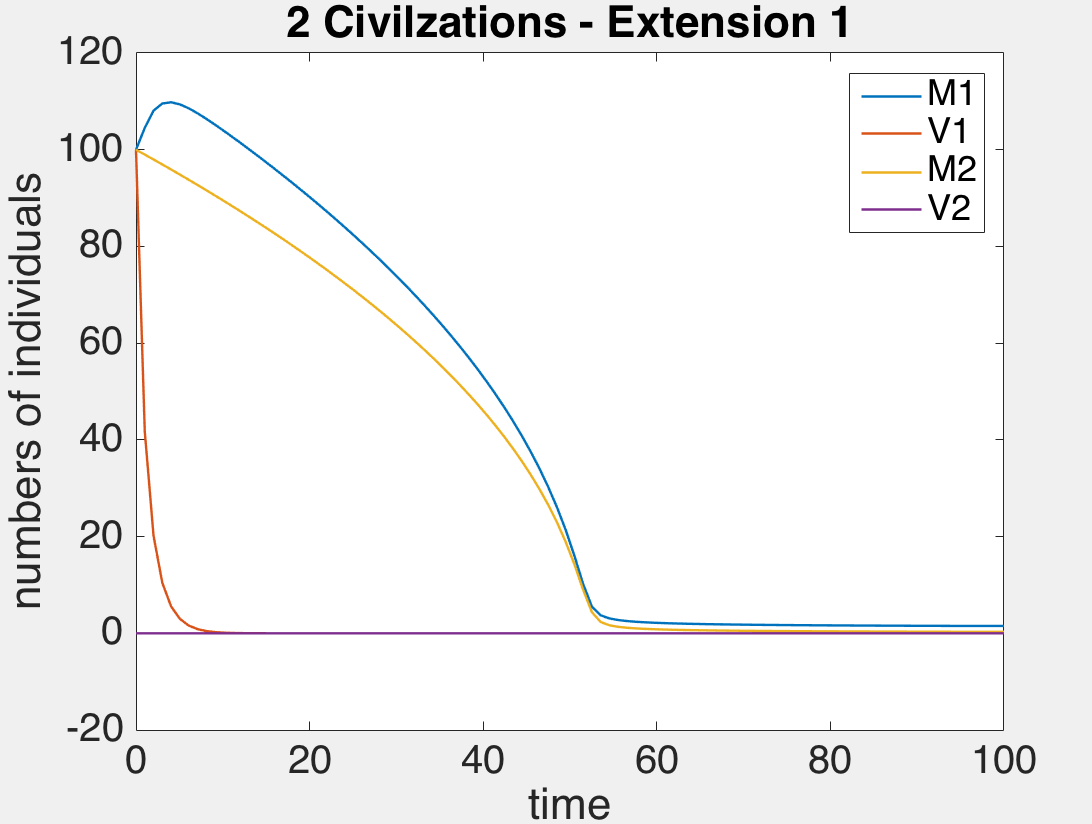
\includegraphics[width=200pt]{examplesim1}
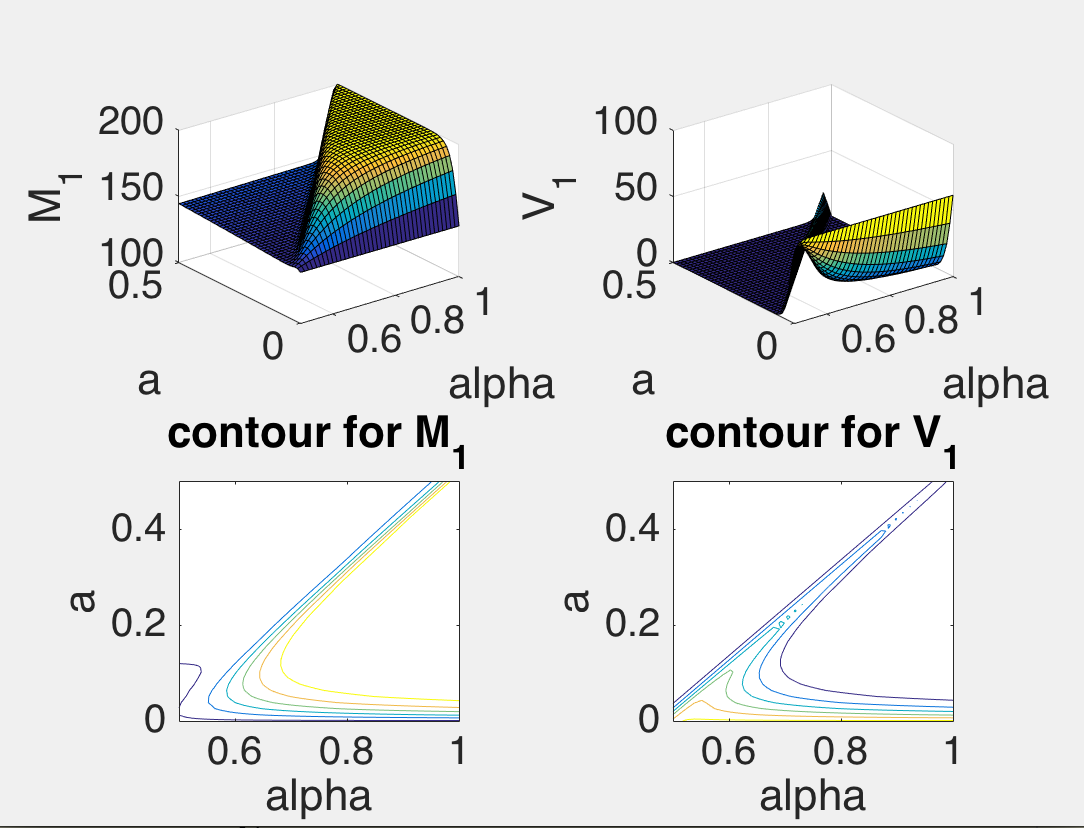
\includegraphics[width=200pt]{examplecontour1}

\subsection{Phase Portraits and Stability Analysis}
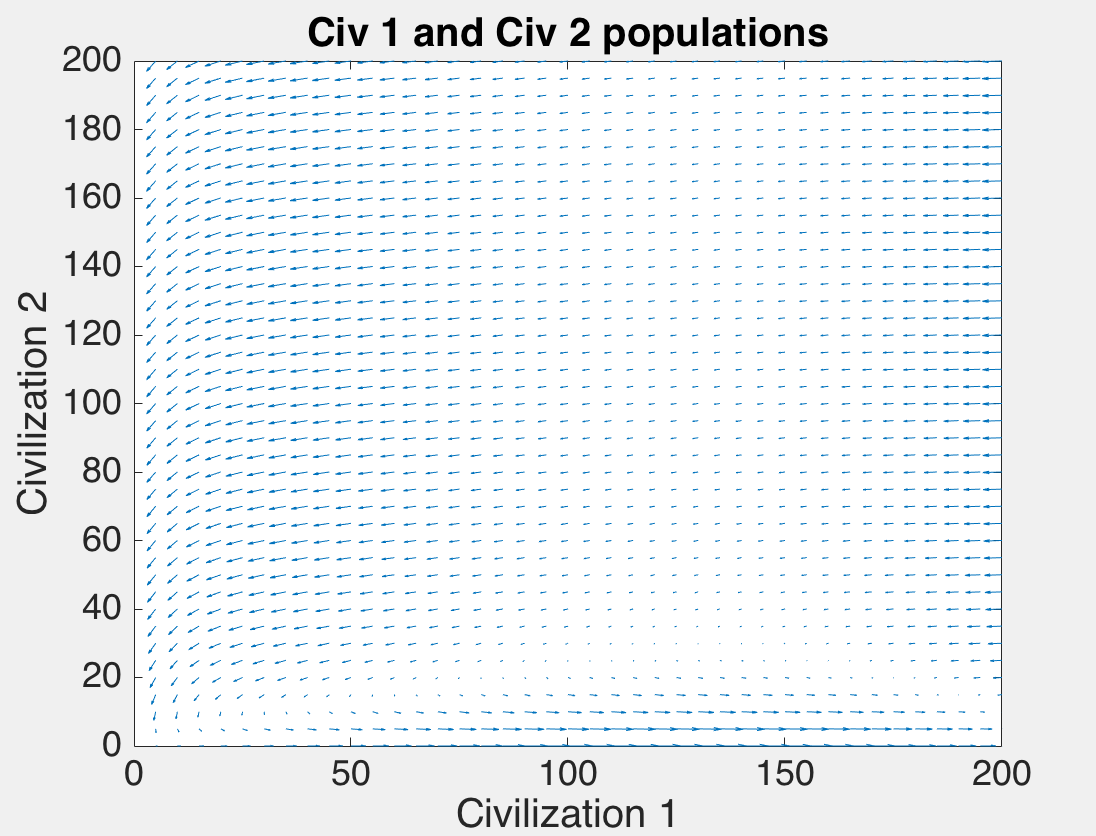
\includegraphics[width=200pt]{phase2}

\subsection{Discussion}

\section{Final Case} 
\paragraph{}
In our final case, we have $C_1 = M_1 + V_1$, with $M_1(0)$ and $V_1(0)$ representing the starting military and villager populations respectively for the first civilzation. However, $C_2 = M_2 + V_2$ as well now, with $M_2(0)$ and $V_2(0)$ representing the starting military and villager populations respectively for the second civilization. \par

We model this case as a set of differential equations: 

$$\frac{dM_1}{dt}=a_1 \alpha V_1(1-\frac{V_1}{K-V_1})-[M_1D_1(\frac{M_2^2}{B+M_2^2})(\frac{M_1}{A+M_1^3})]$$
$$\frac{dV_1}{dt}=(1 - a_1) \alpha V_1(1-\frac{V_1}{K-M_1})-[V_1c D_1(\frac{M_2^2}{B+M_2^2})(\frac{M_1}{A +M_1^2})]$$
$$\frac{dM_2}{dt}=a_2 \beta V_2(1-\frac{V_2}{K-V_2})-[M_2 D_2(\frac{M_1^2}{B+M_1^2})(\frac{M_2}{A +M_2^3})] $$
$$\frac{dV_2}{dt}=(1 - a_2) \beta V_2(1-\frac{V_2}{K-M_2})-[V_2 c D_2(\frac{M_1^2}{B+M_1^2})(\frac{M_2}{A +M_2^2})] $$

Explanation $\cdots$ TODO $c = 6$ because it's easier to kill villagers, specifically in the game miltary units have 6x life points. $\alpha$ and $\beta$ are basically spawn rate params + how quickly you gather resources. It's different for you vs the AI. $a_1$ and $a_2$ is your's vs the AI's strategy of allocating villagers/ military units. 6 PARAMS total.

\subsection{Sensitivity to Parameters}
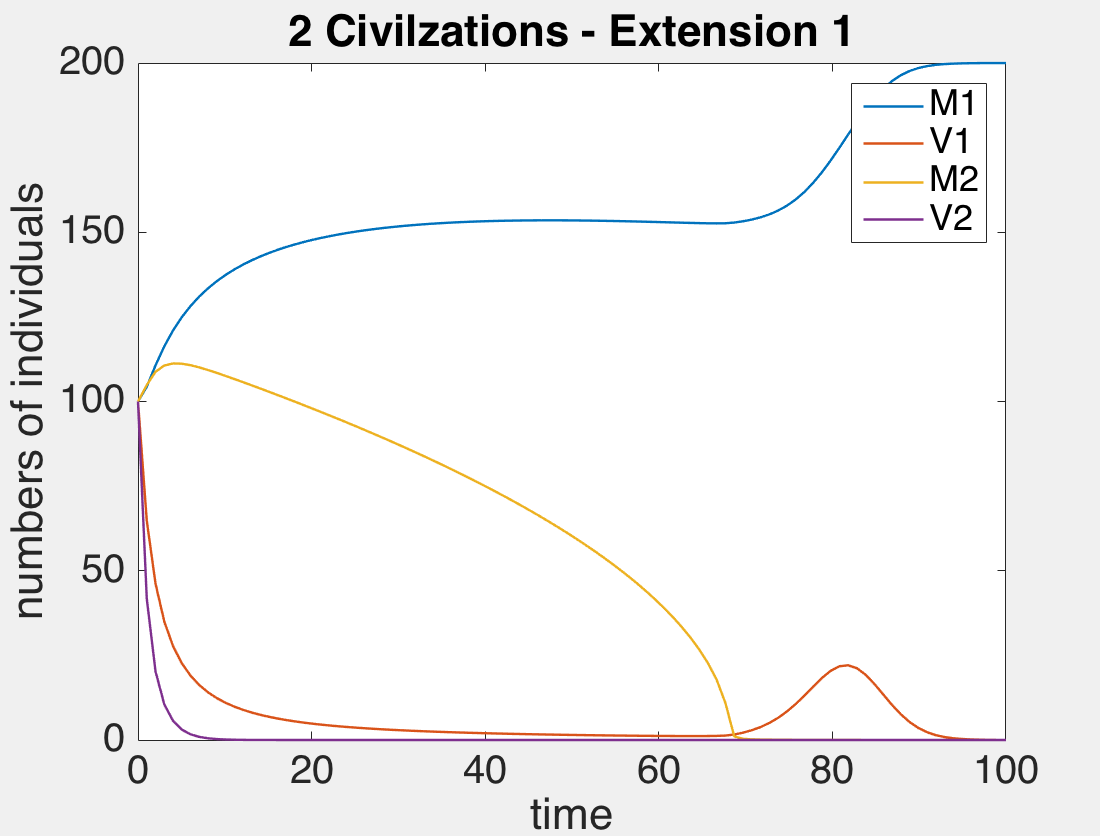
\includegraphics[width=200pt]{examplesim2}

\subsection{Phase Portraits and Stability Analysis}
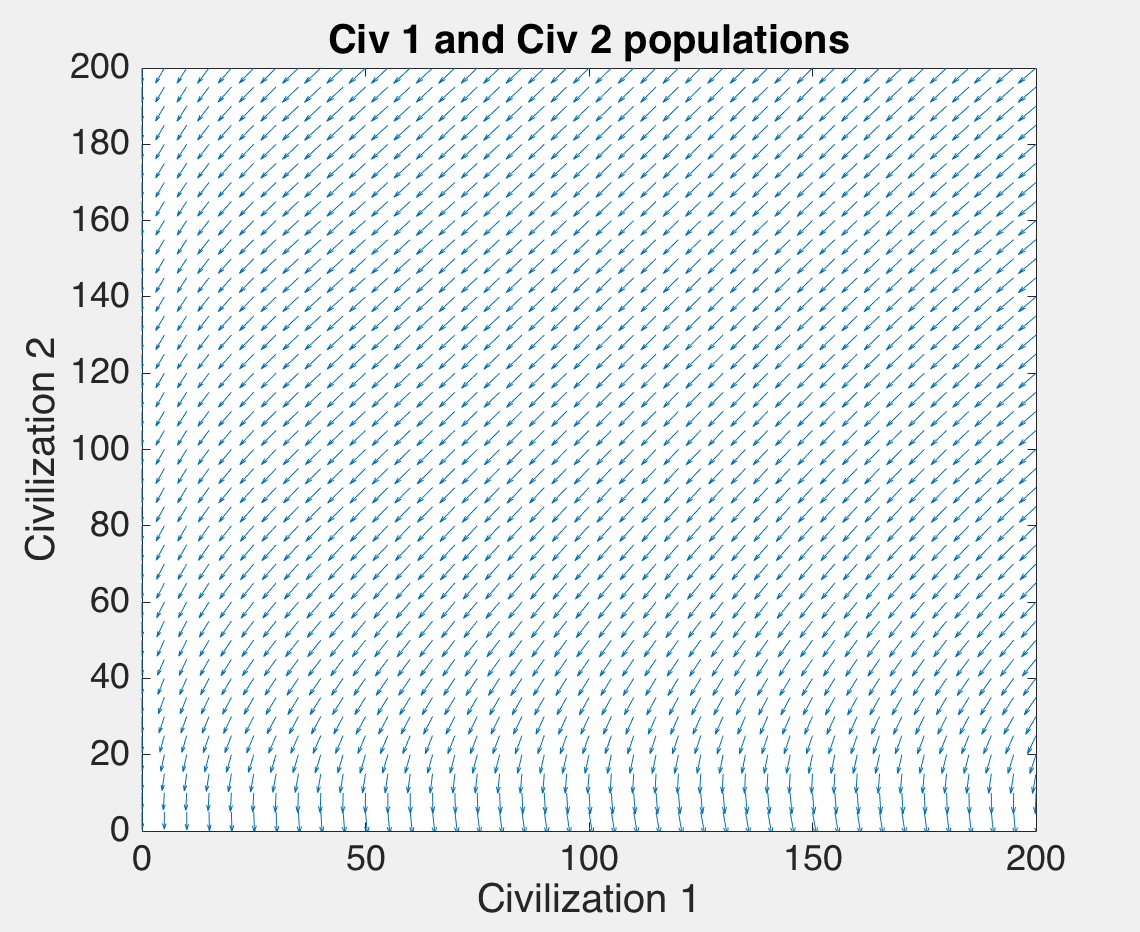
\includegraphics[width=200pt]{phase3}

\subsection{Discussion}

\section{Conclusion} 
\paragraph{}

\section{Attribution of Efforts} 
\paragraph{}

\section{References} 
\paragraph{}

\section{Code Appendix} 
\paragraph{}

\end{document}